\section{Tổng quan cơ sở dữ liệu}

Cơ sở dữ liệu lưu trữ dữ liệu về khách hàng, người dùng, chi nhánh, sản phẩm, tồn kho, đơn hàng,
giữ hàng, giá vốn và các báo cáo cần thiết. Thiết kế ưu tiên tính toàn vẹn, khả năng truy vết
và hiệu năng đối với các thao tác thường xuyên.

\section{Các thực thể chính}

Các thực thể cốt lõi gồm \texttt{Tenant}, \texttt{User}, \texttt{Role}, \texttt{Branch},
\texttt{Category}, \texttt{Brand}, \texttt{Product}, \texttt{Variant}, \texttt{SKU},
\texttt{InventoryLedgerEntry}, \texttt{InventoryBalance}, \texttt{Order}, \texttt{OrderLine},
\texttt{Reservation} và \texttt{CostSnapshot}.

\section{Khách hàng và quyền truy cập}

Mỗi dữ liệu nghiệp vụ thuộc một khách hàng phải mang định danh khách hàng. Người dùng được
liên kết với khách hàng và vai trò. Chi nhánh thuộc một khách hàng và là phạm vi tổ chức của
các hoạt động nhập, chuyển, kiểm kê và bán hàng.

Thiết kế phải bảo đảm định danh của một khách hàng không thể được sử dụng để truy cập dữ liệu
của khách hàng khác. Các khóa ngoại và ràng buộc dữ liệu cần phản ánh quan hệ này.

\section{Mô hình sản phẩm}

Một sản phẩm có thể có nhiều biến thể; mỗi biến thể có thể được biểu diễn bởi một hoặc nhiều
SKU tùy theo mô hình nghiệp vụ. SKU là định danh ổn định để tham chiếu từ tồn kho và dòng đơn
hàng. Mã vạch được lưu để hỗ trợ thao tác tìm kiếm nhanh tại POS.

Giá bán phải được quản lý theo quy tắc thống nhất. Những trường được dùng thường xuyên để tìm
kiếm như SKU, mã vạch và định danh sản phẩm cần được lập chỉ mục.

\section{Sổ cái tồn kho chỉ ghi thêm}

Mỗi biến động tồn kho được ghi thành một bản ghi mới thay vì sửa lịch sử cũ. Bản ghi có thể
chứa SKU, chi nhánh, loại giao dịch, số lượng thay đổi, thời điểm, tham chiếu nghiệp vụ và
người thực hiện.

Các nghiệp vụ nhập hàng, chuyển kho, điều chỉnh kiểm kê, giữ hàng, giải phóng và trừ tồn phải
có dấu vết tương ứng. Nếu cần sửa một nghiệp vụ đã ghi nhận, hệ thống nên tạo giao dịch bù trừ
thay vì xóa lịch sử.

\section{Số dư tồn kho}

Để đọc nhanh, hệ thống duy trì số dư theo SKU và chi nhánh. Các trường quan trọng gồm số lượng
đang có trên thực tế và số lượng đang được giữ. Số lượng có thể bán được tính:

\[
Available = OnHand - Reserved
\]

Bảng số dư là trạng thái phục vụ truy vấn nhanh, trong khi sổ cái là lịch sử biến động có khả
năng kiểm toán.

\section{Đơn hàng và giữ hàng}

Bảng đơn hàng lưu thông tin khách hàng, kênh bán, trạng thái và thời điểm. Bảng dòng đơn hàng
lưu SKU và số lượng. Bảng giữ hàng liên kết đơn hàng với lượng tồn đã giữ tại một chi nhánh.

Thiết kế phải hỗ trợ truy vấn các đơn hàng theo trạng thái, kênh và thời gian; đồng thời hỗ trợ
truy vấn các bản ghi giữ hàng đang còn hiệu lực.

\section{Chỉ mục và toàn vẹn dữ liệu}

Các chỉ mục cần tập trung vào các truy vấn có tần suất cao, đặc biệt là tìm kiếm SKU, mã vạch,
truy vấn tồn theo SKU và chi nhánh, đơn hàng theo trạng thái và thời gian. Các khóa chính, khóa
ngoại, ràng buộc duy nhất và kiểu dữ liệu phải được lựa chọn để hạn chế dữ liệu không hợp lệ.

Các thao tác liên quan đến số dư tồn phải nằm trong giao dịch. Độ chính xác của số lượng và tiền
phải được quy định rõ; các giá trị tiền tệ cần sử dụng kiểu dữ liệu có độ chính xác phù hợp.

\section{Sơ đồ cơ sở dữ liệu}

Hình dưới đây là vị trí dành cho sơ đồ ERD chính thức của dự án. Nhóm bổ sung hình ERD thực tế
sau khi chốt mô hình dữ liệu.

\begin{figure}[H]
    \centering
    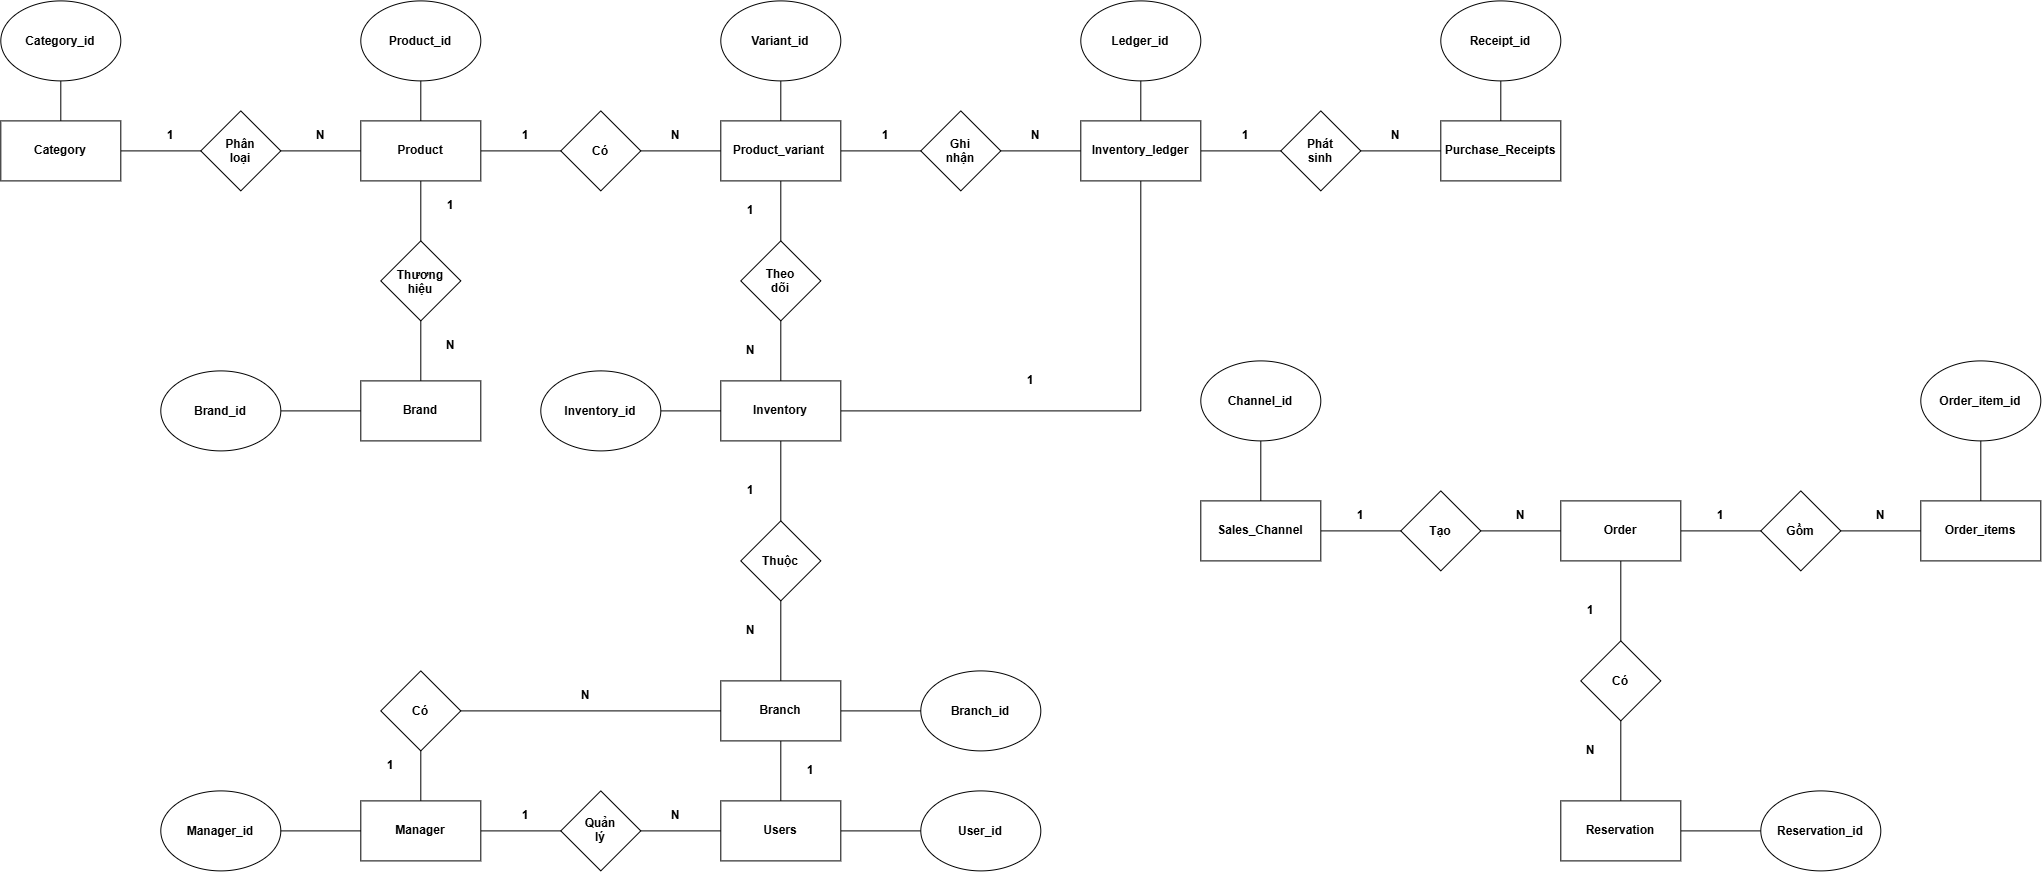
\includegraphics[
        width=0.92\textwidth,
        keepaspectratio
    ]{figures/ERD.png}
    \caption{Sơ đồ ERD cơ sở dữ liệu}
    \label{fig:erd-database}
\end{figure}